\documentclass{article}\usepackage[]{graphicx}\usepackage[]{color}
% maxwidth is the original width if it is less than linewidth
% otherwise use linewidth (to make sure the graphics do not exceed the margin)
\makeatletter
\def\maxwidth{ %
  \ifdim\Gin@nat@width>\linewidth
    \linewidth
  \else
    \Gin@nat@width
  \fi
}
\makeatother

\definecolor{fgcolor}{rgb}{0.345, 0.345, 0.345}
\newcommand{\hlnum}[1]{\textcolor[rgb]{0.686,0.059,0.569}{#1}}%
\newcommand{\hlstr}[1]{\textcolor[rgb]{0.192,0.494,0.8}{#1}}%
\newcommand{\hlcom}[1]{\textcolor[rgb]{0.678,0.584,0.686}{\textit{#1}}}%
\newcommand{\hlopt}[1]{\textcolor[rgb]{0,0,0}{#1}}%
\newcommand{\hlstd}[1]{\textcolor[rgb]{0.345,0.345,0.345}{#1}}%
\newcommand{\hlkwa}[1]{\textcolor[rgb]{0.161,0.373,0.58}{\textbf{#1}}}%
\newcommand{\hlkwb}[1]{\textcolor[rgb]{0.69,0.353,0.396}{#1}}%
\newcommand{\hlkwc}[1]{\textcolor[rgb]{0.333,0.667,0.333}{#1}}%
\newcommand{\hlkwd}[1]{\textcolor[rgb]{0.737,0.353,0.396}{\textbf{#1}}}%
\let\hlipl\hlkwb

\usepackage{framed}
\makeatletter
\newenvironment{kframe}{%
 \def\at@end@of@kframe{}%
 \ifinner\ifhmode%
  \def\at@end@of@kframe{\end{minipage}}%
  \begin{minipage}{\columnwidth}%
 \fi\fi%
 \def\FrameCommand##1{\hskip\@totalleftmargin \hskip-\fboxsep
 \colorbox{shadecolor}{##1}\hskip-\fboxsep
     % There is no \\@totalrightmargin, so:
     \hskip-\linewidth \hskip-\@totalleftmargin \hskip\columnwidth}%
 \MakeFramed {\advance\hsize-\width
   \@totalleftmargin\z@ \linewidth\hsize
   \@setminipage}}%
 {\par\unskip\endMakeFramed%
 \at@end@of@kframe}
\makeatother

\definecolor{shadecolor}{rgb}{.97, .97, .97}
\definecolor{messagecolor}{rgb}{0, 0, 0}
\definecolor{warningcolor}{rgb}{1, 0, 1}
\definecolor{errorcolor}{rgb}{1, 0, 0}
\newenvironment{knitrout}{}{} % an empty environment to be redefined in TeX

\usepackage{alltt}
\usepackage[utf8]{inputenc}
\usepackage[spanish]{babel} 
\usepackage{subcaption}
\usepackage{multirow}
\usepackage{hyperref}
\usepackage{amssymb}
\usepackage{enumitem}
\hypersetup{
    colorlinks,
    citecolor=black,
    filecolor=black,
    linkcolor=black,
    urlcolor=black
}
\usepackage{graphicx}
\usepackage{geometry}
 \geometry{
 a4paper,
 left=20mm,
 right=20mm,
 bottom=30mm,
 top=30mm,
 }
\title{
    \textbf{UNIVERSIDAD DE ALCAL\'A}\\
    Escuela Polit\'ecnica Superior~\\~\\~\\
    \textbf{GRADO EN INGENIER\'IA INFORM\'ATICA}~\\~\\
    Trabajo de Fin de Grado~\\
    \textbf{Estado del arte de visualizaci\'on circular de datos con R}~\\~\\~\\
    \textbf{Autor:} Pablo Garc\'ia Lacalle ~\\
    \textbf{Tutor:} Juan Jos\'e Cuadrado Gallego~\\~\\~\\
    \textbf{TRIBUNAL}~\\~\\
    \begin{flushleft}
    \textbf{      Presidente:}~\\
    \textbf{      Vocal 1:}~\\
    \textbf{      Vocal 2:}~\\~\\
    \textbf{Calificaci\'on: }
    \end{flushleft}
}
\author{}
\date{}
\IfFileExists{upquote.sty}{\usepackage{upquote}}{}
\begin{document}
 \renewcommand{\labelitemi}{$\bullet$}
 \renewcommand\labelitemii{$\circ$}
\vbox{
    \centering
    
\includegraphics[width=0.6\textwidth]{imag/logo}
    \maketitle %this typesets the contents of \title, \author and \date
}
\tableofcontents
~\\~\\~\\~\\~\\~\\~\\
\section*{Resumen}
Este trabajo realiza una estudio de que tipos de diagramas con formato circular existen, y como realizarlos con el lenguaje de programaci\'on destinado a estad\'istica R\cite{R}
. Para ello se necesita explorar los tipos de diagramas circulares gracias a  libros, como "The Book of Circles, Visualizing Spheres of Knowledge" de Manuel Lima\cite{Circle}
, "Information Graphics, A Comprehensive Ilustrated Reference" de Robert L. Harris\cite{Info}
.
Y saber qu\'e paquetes de R se pueden utilizar para representar dichos gr\'aficos. Para una correcta representaci\'on de los diagramas en c\'odigo, es muy recomendable la lectura de "Data Visualization, A Practical Introduction"de Kieran Healy\cite{Data}
.
\markboth{RESUMEN}{RESUMEN} 
\clearpage
\section{Introducci\'on}
El mundo est\'a repleto de datos obtenidos de la observaci\'on, experimentos, etc. Pero, estos por si solos, no aportan el conocimiento necesario para que sus receptores saquen informaci\'on v\'alida.~\\
Dicha informaci\'on ayuda a la capacidad de entender el entorno que nos rodea (f\'isica, biolog\'ia, geolog\'ia, etc) y para ser capaces de realizar una mejor toma de decisiones (pandemias, econom\'ia, etc).
Pero, para transformar estos datos en informaci\'on v\'alida, hay que condensarlos en una representaci\'on gr\'afica que ayude a, la interpretaci\'on y construcci\'on de signaificado de los datos, y a la comunicaci\'on de la informaci\'on obtenida.~\\
Por ejemplo, si se tienen muchos datos con los sueldos de los habitantes de un pa\'is y se transforman siguiendo la estad\'istica, se puede obtener el sueldo medio de \'este junto con la moda del sueldo, etc; para que el pa\'is tome la decisiones pertinentes con dicha informaci\'on.~\\
Para cada situaci\'on existe un tipo de visualizaci\'on de datos: para n\'umeros las tablas; para comparar informaci\'on de diferentes entidades en un instante de tiempo las barras; para visualizar cambios a lo largo del tiempo u otra variable, las l\'ineas; etc.~\\~\par
Todas estas variedades de visualizaciones se pueden, como  es objetivo de este trabajo, realizar con un formato de c\'irculos. Estos son una de las figuras geom\'etricas que m\'as fascinan a la humanidad, debido a que se vislumbraban con mucha facilidad en la naturaleza, como astros celestiales, lagos, ondas generadas en el agua, frutas, etc.~\\~\par
Los c\'irculos empezaron a usarse en arquitectura, por ejemplo, en b\'ovedas; en ciudades, como las aldeas de nativos americanos; en fortificaciones, como la muralla de \'Avila (Espa\~na); met\'aforas universales, como de la perfecci\'on (God the Architect, William de Bailes), la unidad (Fra Mauro map, Fra Mauro), el movimiento (Yama holding the wheel of life), la infinidad (Miracles of Each Moment); en mucha de la simbolog\'ia como , la representaci\'on del tiempo, el ciclo de la vida, en los logos de empresas como, Vodafone, Bayer, Motorola, Mercedes; y en simbolog\'ia antigua como los petroglifos prehistoricos de Argyll \cite[p\'ag 15-54]{Circle}
.~\\~\par
Los humanos est\'an constantemente buscando patrones, orden, pautas, instruciones, debido a ello consiguen compreder mejor lo que les rodea, como los seres vivos (biolog\'ia), seres inertes, lo terrenal, lo espacial y en general, los patrones que gobiernan el universo. Y gracias al formato circular de los diagramas, que se representar\'an a lo largo de este trabajo, se pueden identificar dichas pautas, normalmente c\'iclicas, en los diferentes datos que recreen los distintos diagramas.~\\~\par
Para este trabajo se ha optado por R\cite{R}
, lenguaje de programaci\'on con enfoque estad\'istico basado en software libre, donde cada persona pueda contribuir a su crecimiento mediante un conjunto de funciones agrupadas en paquetes. Este lenguaje es uno de los m\'as usados para Big Data, miner\'ia de datos, matem\'aticas financieras, aprendizaje autom\'atico, etc. En este caso, se trabaja en el \'area de Big Data con la visualizaci\'on de datos, por lo que estos diferentes diagramas ayudan a la observacion y comprensi\'on de grandes cantidades de datos.
\clearpage
\subsection{Visualizaci\'on de Datos}
Visualizar: Representar mediante im\'agenes \'opticas fen\'omenos de otro car\'acter\cite{rae}
, por consiguiente, la visualizaci\'on de datos es la representaci\'on gr\'afica de datos. Lo que implica producir im\'agenes que comunican relaciones entre los datos representados a los observadores. Refiri\'endose a las t\'ecnicas usadas para comunicar datos o informaci\'on mediante su codificaci\'on como objetos visuales (puntos, barras, l\'ineas, etc.) contenidos en un gr\'afico.~\\
"La meta principal de la visualizaci\'on de datos es comunicar informaci\'on clara y efectivamente gracias a medios gr\'aficos. Esto no significa que la visualizaci\'on de datos necesite parecer aburrida para ser pr\'actica o extremadamente sofisticada para parecer bonita. Para transmitir ideas de forma eficiente, tanto la est\'etica como la funcionalidad necesitan ir de la mano, proporcionando informaci\'on sobre un conjunto de datos escasos y complejos mediante la comunicaci\'on de sus aspectos clave de una manera m\'as intuitiva. Todav\'ia los dise\~nadores suelen fallar a alcanzar un balance entre la forma y la funci\'on, creando bellas visualizaciones de datos que erran el prop\'osito general de comunicar informaci\'on"\cite[Vitaly Friedman]{vitaly}
. "Hechas bien, las visualizaciones explicar complejas ideas de manera simple"\cite[Thomas Powell, CEO de ZingChart]{zingchart}
.~\\~\par
Una visualizaci\'on ideal no solo debe comunicar de forma clara, sino que se necesita estimular compromiso y atenci\'on al espectador\cite{sexy}
. Por ello se considera a la visualizaci\'on de datos arte aparte de ciencia\cite{moma}\cite{art}
.~\\
Durante su historia, este campo y sus profesionales han abordado distintos tipos de retos tanto \'eticos como anal\'iticos\cite{history}
, debido a esto se ha vuelto un \'area activa en la investigaci\'on, el desarrollo y la ense\~nanza\cite{articulos}
.~\\~\par
Los gr\'aficos (de barras, l\'ineas, puntos, etc.) usados en la visualizaci\'on m\'as tradicional (horizontal) suelen estar construidos con un sistema de coordenadas cartesianas\cite{coord_carte}
.~\\
\begin{knitrout}
\definecolor{shadecolor}{rgb}{0.969, 0.969, 0.969}\color{fgcolor}

{\centering 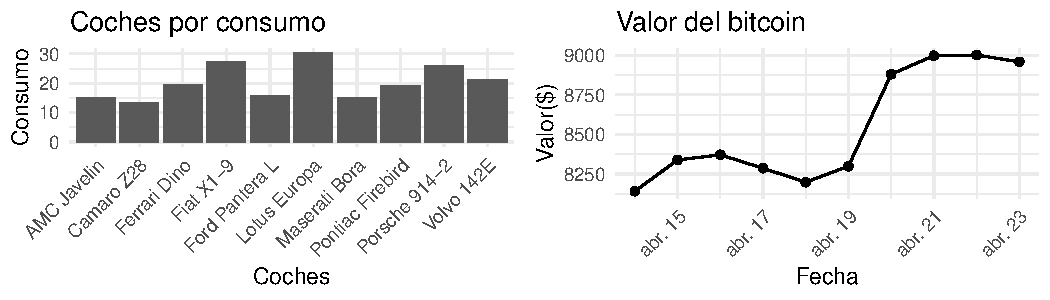
\includegraphics[width=\maxwidth]{figure/examples_carte-1} 

}



\end{knitrout}
Pero para este trabajo se interesa en los gr\'aficos que se pueden construir con un formato circular mediante el cambio del sistema de coordenadas a las polares\cite{coord_polar}
. Este formato ayuda a la comprensi\'on en algunos conjuntos de datos, su estructura, comparaciones y relaciones. Este sistema en ocasiones ayuda a la atenci\'on del espectador, pero en algunas, como se dijo antes, lleva a cometer el fallo de crear gr\'aficos m\'as est\'eticos que funcionales, olvidando la meta de comunicar informaci\'on de forma clara y eficaz.~\\~\par
Sin embargo, este formato de visualizaci\'on de datos con formato circular, si se usa bien, es uno de los formatos m\'as eficientes para expresar estructuras jer\'arquicas, sus relaciones, realizar comparaciones sencillas de agrupaciones de datos para exponer un patr\'on. Esto se hace notar m\'as con los diagramas de \'arbol y redes por el hecho de no necesitar tanto espacio, comparado con su formato de sistema de coordenadas cartesianas. Otro buen grupo de datos para exponer en un c\'irculo son los datos porcentuales, con no gran cantidad de porcentajes parecidos, para ellos siempre es necesario el uso de una leyenda o cualquier informaci\'on a\~nadida que ayude a la comprensi\'on del diagrama.
\clearpage
En algunos casos la eficiencia ofrecida por el formato circular solo recae en el tama\~no que ocupa el diagrama al exponerlo de esta forma, como por ejemplo los diagramas de barras o columnas, pero a la hora de comparar resultados de forma m\'as r\'apida esta manera de representar decae con respecto a su formato cartesiano.~\\~\par
Pero la mayor ventaja del formato circular es su capacidad de atraer la atenci\'on del espectador, debido a que a los seres humanos, seg\'un un estudio[cita psic\'ologo], nos atraen las formas curvas por el hecho de no asociarlas a objetos afilados que puedan ser un riesgo para la supervivencia.~\\
Por lo que el c\'irculo como formato para visualizar datos cumple la meta de la visualizaci\'on, si se usan los datos y tipos de diagramas adecuados, de ser capaz de transmitir informaci\'on al observador de forma clara, efectiva de manera que la informaci\'on atraiga y se quede con ellos un mayor periodo de tiempo.~\\~\par
Para ello es necesario presentar el c\'irculo y sus partes para entender c\'omo se construyen.
~\\
\subsection{C\'irculos}
El c\'irculo es un \'area o superficie plana contenida dentro de una circunferencia\cite{rae}
, o tambi\'en se puede definir como un conjunto de puntos en un plano equidistantes de un punto dado, llamado centro\cite{circulo}.~\\
Los elementos esenciales para comprender los diagramas y explicaciones del trabajo son:
\begin{itemize}
\item \textbf{Centro}:~\par Punto fijo interior, equidistante de su per\'imetro a una distancia igual al radio.
\item \textbf{Radio}:~\par Segmento que une el centro del c\'irculo con cualquier punto del per\'imetro de este.
\item \textbf{Cuerda}:~\par Segmento que une dos puntos del per\'imetro del c\'irculo sin pasar por el centro.
\item \textbf{Arco}:~\par Es la parte del per\'imetro del c\'irculo que resulta entre dos extremos de una cuerda.
\item \textbf{Sector circular}:~\par Parte del c\'irculo comprendida entre dos radios y el arco que delimitan.
\item \textbf{C\'iculos conc\'entricos}:~\par Dos o m\'as c\'irculos con mismo centro y distinto radio.
\item \textbf{Corona circular}:~\par Superficie del c\'irculo comprendida entre dos c\'irculos conc\'entricos.
\end{itemize}
\clearpage
\section{A\'nalisis de los Diagramas}\label{sec:Analisis}
Para poder usar cada uno de los diagramas, es necesario comprender sus virtudes, sus defectos y como se estructuran los datos para depu\'es elegir el m\'as adecuado.~\\
En esta secci\'on se estudia la definici\'on de los diagramas, c\'omo y de qu\'e se componen , para poder identificar despu\'es qu\'e paquetes de R pueden implementar dichos diagramas sus ventajas e inconvenientes a la hora de visualizar los datos requeridos respecto a otros formatos.~\\
Esta selecci\'on de diagramas circulares se han escogido siguiendo el libro de Manuel de Lima\cite{Circle}
, donde se presenta una clasificaci\'on diferenciada en familias seg\'un la similaridad de construcci\'on.~\\ Estos se agrupan en siete familias:

\begin{itemize}
\item Familia de anillos y espirales. Estos diagramas presentan patrones de c\'irculos conc\'entricos.
\begin{itemize}
  \item Diagrama de Anillos.
  \item Diagrama de Barras Radiales.
  \item Diagrama en Espiral.
\end{itemize}
\item Familia de ruedas y tartas. Los diagramas que forman esta familia presentan patrones de l\'ineas radiales.
\begin{itemize}
  \item Diagrama de Columnas Radiales.
  \item Diagrama de Sectores.
  \item Diagrama Rose of Nightingale.
\end{itemize}
\item Familia de cuadr\'iculas y ret\'iculas. La forman diagramas de cuadr\'iculas circulares.
\begin{itemize}
  \item Diagrama de Cuadr\'icula Circular Ordenada.
  \item Diagrama de Cuadr\'icula Circular Desordenada.
  \item Diagrama  Rayos de Sol.
\end{itemize}
\item Familia de flujos. Los diagramas que la conforman tienen patrones de flujo radiales con barras y l\'ineas.
\begin{itemize}
  \item Diagrama  Radar.
  \item Diagrama de Columnas con Formato Iris.
  \item Diagrama de L\'ineas Circulares Multiseries.
\end{itemize}
\item Familia de formas y l\'imites. En estos diagramas se delimita, con alguna variable, la forma de los objetos y sus l\'imites.
\begin{itemize}
  \item Diagrama de Burbujas.
  \item Diagrama de Mapa de \'Arbol Circular.
  \item Diagrama de Mapa de \'Arbol Voronoi.
\end{itemize}
\item Familia de mapas y planos. El propio nombre de la familia indica que tipo de diagramas se concentran en esta.
\begin{itemize}
  \item Diagrama de Planos Circulares.
  \item Diagrama Mapa Circular.
  \item Diagrama Mapa de Esfera.
\end{itemize}
\item Familia de nodos y enlaces. Estos diagramas usan patrones de tipo \'arbol y redes.
\begin{itemize}
  \item Dendograma Circular.
  \item Diagrama de Cuerdas.
  \item Diagrama de Redes Circulares.
\end{itemize}
\end{itemize}
\subsection{Diagrama de Anillos}~\par
El diagrama de Anillos consiste en una divisi\'on de c\'irculos conc\'entricos, resultando en varias coronas circulares en las que en cada una se pueden visualizar diferentes conjuntos de datos.~\\~\par
La estructura de este diagrama, al consistir en varias coronas circulares, puede representar diferentes variables, diferentes tipos de gr\'afico o diferentes conjuntos de datos como, por ejemplo, el uso del ancho de las coronas puede ser preestablecido por una variable mientras el color de cada anillo por otra. Pero tambi\'en se pueden crear diferentes tipos de gr\'aficos en cada corona, por ejemplo, representando un espacio de tiempo en los datos de cada c\'irculo.~\\~\par
La primera forma comentada se construye dividiendo el c\'irculo principal, el que encapsula el gr\'afico, en tantas coronas como entidades se quieran representar y ajustando su tama\~no (\'area)  mediante una variable representada de forma proporcional, estableciendo el radio total del c\'irculo como el 100\%. Otra caracter\'istica a tener en cuenta es la agrupaci\'on de las entidades representadas, se\~naliz\'andolas mediante el color de las coronas circulares. Aunque como en esta variante ya es una agrupaci\'on\cite{Jax_de_leon} no se suele ver agrupaci\'on por colores.~\\~\par
La segunda forma al consistir en diferentes gr\'aficos en cada corona se puede construir o usando deferentes tipos de gr\'aficos en cada corona como l\'ineas, puntos, barras…, o con el mismo tipo de gr\'afico, pero con distintos grupos de datos. Esta forma es \'util para presentar comparaciones entre los diferentes conjuntos de datos\cite[Figura 1-F]{genoma} o comparar diferentes formas de representar los mismos datos\cite{cultivation}.~\\~\par
Existe otra variaci\'on de este tipo de diagramas, llamado diagrama de cebolla\cite{cebolla} donde se representan conjuntos de datos y sus relaciones, como estructuras jer\'arquicas. Este diagrama se construye (con jerarqu\'ia) exponiendo la ra\'iz de los datos en la corona interior, y seg\'un los niveles de descendencia de los datos con la ra\'iz se colocan en las coronas m\'as o menos exteriores o exponiendo una entidad en la corona interior y posicionar las dem\'as en las distintas coronas dependiendo de su relaci\'on con la interior\cite{cebolla_biogas}\cite{cebolla_cultura}.~\\~\par
El problema con este diagrama es que la perspectiva de las coronas seg\'un su posici\'on (interior o exterior), dificulta la comprensi\'on. Si, por ejemplo, los mismos datos se implementan en una corona exterior, resultar\'an con m\'as magnitud que la que se sit\'ua en una interior.
~\\~\\~\\~\\
\vbox{
    \centering
    
\includegraphics[width=0.25\textwidth]{imag/anillos}
}
\clearpage
\subsection{Diagrama de Barras Radiales}\label{ssec:barras}
El diagrama de Barras Radiales, o tambi\'en llamado diagrama de Barras Circulares, es un gr\'afico de barras en el que, en lugar de usar un sistema de coordenadas cartesianas como el horizontal, se usa el sistema de coordenadas polares, situando las categor\'ias a representar en el eje Y.~\\~\par
El diagrama de barras es un gr\'afico que representa valores num\'ericos de categor\'ias discretas mediante barras rectangulares para su comparaci\'on. Ajustando la longitud de la barra al valor seg\'un la escala de valores que se est\'e usando[cita historia-barras].~\\~\par
Si se quiere representar un valor por cada categor\'ia discreta las barras pueden ser organizados de diferentes maneras, como siguiendo un orden del eje donde est\'en las categor\'ias discretas, por ejemplo, meses del a\~no; el orden de las barras se puede ordenar dependiendo de la longitud de ellas (ascendente o descendente); o agruparlas seg\'un una variable y a su vez estos grupos se pueden ordenar como las otras dos formas.~\\~\par
Sin embargo, para m\'ultiples valores por categor\'ia discreta, existe la variante de barras apiladas, que consiste en, como su nombre indica, apilar las barras de la misma categor\'ia creando una barra final dividida en tantos valores como se quieran exponer.~\\~\par
La estructura de este gr\'afico se crea con las barras formando c\'irculos conc\'entricos sobre el c\'irculo que act\'ua como plantilla, donde los divisores radiales sirven para marcar la longitud de las barras.~\\~\par
Esta estructura tiene el mismo problema de malinterpretaci\'on de los valores. \'este radica en que, al ser el radio de cada barra diferente dependiendo de qu\'e posici\'on ocupa en la plantilla, si se observan dos barras con valores iguales, la que est\'e posicionada en la parte exterior se interpreta como mayor magnitud que la que est\'a en la parte interior. Es por eso por lo que este diagrama, se suelen ordenar las barras (si el eje de categor\'ias permite reordenaci\'on) descendentemente de fuera a dentro, pero se usa m\'as con prop\'ositos est\'eticos que pr\'acticos, para cautivar m\'as al observador.
~\\~\\~\\~\\
\vbox{
    \centering
    
\includegraphics[width=0.25\textwidth]{imag/barras_radiales}
}
\clearpage
\subsection{Diagrama en Espiral}
El diagrama en Espiral consiste en un gr\'afico que expone los datos requeridos datos con la forma de una espiral gracias a una variable. La espiral se puede definir como, una curva que da vueltas indefinidamente alrededor de un punto, alej\'andose de \'el m\'as, en cada una de ellas\cite{rae}.~\\~\par
Esta espiral se puede construir de muchas formas adecu\'andose a la funci\'on de su realizaci\'on: La espiral de Arqu\'imedes ($r = a\theta$)\cite{mat_arqui}, logar\'itmica ($r=a e^{b\theta}$)\cite{mat_log}, la espiral de Theodorus\cite{mat_theo}, hiperb\'olica ($r=  a/\theta$)\cite{mat_hiper}, la espiral prime\cite{mat_prime}, etc.( r es la distancia de un punto al origen, $\theta$ es el \'angulo con respecto al eje X y a,b son constantes arbitrarias).~\\~\par
Cualquier espiral se construye estableciendo el eje X a la forma de la espiral teniendo sus valores, continuos o discretos, ordenados siguiendo alg\'un tipo de criterio, como el peso at\'omico de los elementos de la tabla peri\'odica\cite{tipos_espiral}.~\\~\par
Aunque donde destaca este diagrama es con la representaci\'on de conjuntos de datos de series de tiempo, es decir, escogiendo el valor a exponer en la espiral el tiempo en que se recogen los datos. Las espirales en este aspecto, de visualizar datos con variable temporal ofrece una serie de ventajas que otros tipos de diagramas no, como: proporcionar una t\'ecnica de visualizaci\'on apropiada para datos nominales, ordinales y cuantitativos; soporta la visualizaci\'on de grandes cantidades de datos; soporta la lectura comparativa del conjunto de datos; soportar el an\'alisis de los datos en nivel resumido, facilidad de detectar patrones; permitir la comparaci\'on de m\'ultiples conjuntos de datos\cite{espiral}.~\\~\par
Este gr\'afico se usa primordialmente para representar el paso del tiempo en un conjunto de datos, haciendo coincidir el origen de la espiral con el comienzo temporal de los datos; una vez establecida la variable para el eje X se necesita que alg\'un dato se refleje en el tiempo, eje Y, para ello, se suelen usar barras, l\'ineas o puntos para dibujar los datos que se exponen, dividi\'endolos en rangos de tiempo para que resulten m\'as f\'aciles de leer e implementar. Se puede dar otra dimensi\'on al diagrama usando el color para expresar otra variable y as\'i ayudar a la visualizaci\'on.~\\~\par
Otra forma de crear estas espirales es gracias a la interactividad, que ofrecen algunos paquetes del lenguaje R, ayudando a la ampliaci\'on de la informaci\'on que puede representar el diagrama\cite{espiral_inte}.~\\~\par
Este gr\'afico es unos de los m\'as \'utiles para mostrar c\'omo se actualizan los datos en cada rango de tiempo, siendo ideal para detectar tendencias, patrones peri\'odicos gracias a los ciclos que realiza la espiral, normalmente haciendo coincidir cada vuelta al c\'irculo plantilla con un periodo de tiempo concreto, o medida peri\'odica de la variable representada en el eje X.
~\\~\\~\\~\\
\vbox{
    \centering
    
\includegraphics[width=0.25\textwidth]{imag/espiral}
}
\clearpage
\subsection{Diagrama de Columnas Radiales} \label{ssec:colRadiales}
Este diagrama, llamado de Columnas Radiales, de Columnas Circulares o de Estrella, es otra de las formas de crear un gr\'afico de barras con coordenadas polares, pero esta vez con el eje X es el que act\'ua como el eje de las categor\'ias.~\\~\par
Aunque este diagrama es llamado de columnas, esto es solo porque al diagrama de barras se le conoce como de columnas cuando las barras est\'an situadas verticalmente. Y como se ha explicado en \ref{ssec:barras}, se utiliza como plantilla el diagrama de barras, exponiendo valores num\'ericos de categor\'ias discretas para su comparaci\'on[cita historia-barras].~\\~\par
En este caso, los divisores radiales se convierten en las barras y la magnitud se calcula con la distancia del centro a su punto m\'as exterior. Debido a su formato circular es muy recomendable que el diagrama tenga una buena cuadr\'icula para la correcta medici\'on de los valores de las columnas. Estas columnas tambi\'en se pueden representar, al igual que las barras, como columnas apiladas para visualizar m\'as cantidad de valores por categor\'ia discreta.~\\~\par
Este gr\'afico tiene un problema con la dificultad con la que se visualiza la informaci\'on, ya que nunca va a ser tan claro destacar una barra en un gr\'afico con coordenadas polares como uno con cartesianas. Por su modificaci\'on de los ejes de coordenadas cada barra, a no ser que destaque, solo se puede comparar con las pocas barras alrededor a simple vista y para la comparaci\'on con todas ellas es necesario estar utilizando la cuadr\'icula donde se expone la escala de valores.
~\\~\\~\\~\\
\vbox{
    \centering
    
\includegraphics[width=0.25\textwidth]{imag/columnas}
}
\clearpage
\subsection{Diagrama de Sectores}
El diagrama de Sectores o de Tarta es uno de los m\'as conocidos y empleados (empresas, oficinas, etc.), pero algunos expertos opinan que este tipo de diagramas son malos a la hora de representar informaci\'on de forma eficiente, ya que solo son efectivos en situaciones donde se muestran magnitudes porcentuales de 25, 50, 75, 100. Pero cuando se trata de crear gr\'aficos con valores porcentuales que sean m\'as cercanos entre ellos, es mejor usar un diagrama de barras\cite{pie-bad}.~\\~\par
Sin embargo, este diagrama tiene la ventaja de ser entendido por cualquier observador sin necesidad de conocimiento del diagrama, por el uso de estos diagramas para aprender las fracciones en la ni\~nez\cite{save-pie}. Y se aumenta la comprensi\'on del diagrama con muchos datos con la ayuda de la interactividad o las etiquetas para representar los valores de forma clara. Esto se puede relacionar con la tipograf\'ia Comic Sans (dise\~nada para que se pareciera a una tipograf\'ia de comic en un entorno poco definido, pero que se entendiera claramente), porque esta al igual que el diagrama se creo para situaciones espec\'ificas, aunque se ha usado y se usar\'a de forma inadecuada para las situaciones a exponer.~\\~\par
Este gr\'afico se lleva usando para la visualizaci\'on de datos desde hace 200 a\~nos (Playfair, 1801). Y se populariz\'o m\'as tarde por la sencillez de entender este diagrama circular por gran cantidad de personas con diferente educaci\'on. Pero sin dejar de lado sus cr\'iticas por ser ineficaz para representar muchos datos y se recomienda dejar de usar para los negocios\cite{humble-pie}.~\\~\par
El diagrama se construye dividiendo el c\'irculo plantilla de forma proporcional, al igual que el diagrama de Anillos, pero en vez de dividirlo con las coronas circulares se opta por sectores circulares, estableciendo la longitud del arco del sector de manera proporcional siendo el 100 \% con los 360 grados del c\'irculo, resultando como su nombre dice en pedazos de una tarta.~\\~\par
Su principal ventaja es que es muy \'util para visualizar la distribuci\'on proporcional de un conjunto de datos. Pero el problema de este tipo de diagrama es que no se pueden representar grandes cantidades de datos, porque se perder\'ia la ventaja de f\'acil visualizaci\'on de la informaci\'on. Tambi\'en es dif\'icil hacer comparaciones entre varios gr\'aficos de sectores.~\\~\par
Hay variantes de este diagrama que ayudan a concentrar la atenci\'on del p\'ublico en los datos deseados como el diagrama de sectores donde estos se separan del centro como en una explosi\'on\cite{pie-explode}, con otra dimensi\'on realizando un diagrama de sectores en 3-D (resultando en ninguna informaci\'on a\~nadida, por lo que solo es por est\'etica), y de este diagrama se han derivado otro tipo de ellos que se explicar\'an m\'as tarde como el diagrama de Rayos de Sol o el diagrama Rose of Nightingale.~\\~\par
Existe una variante de este diagrama que se construye y funciona de la misma forma que el de sectores, pero quitando un c\'irculo conc\'entrico con un radio m\'as peque\~no que el de plantilla, dejando un espacio en el centro, usado normalmente para a\~nadir informaci\'on como el t\'itulo o leyenda si encaja en el espacio. Esta variante se llama el diagrama donut.
~\\~\\~\\~\\
\vbox{
    \centering
    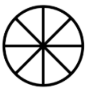
\includegraphics[width=0.25\textwidth]{imag/sectores}
}
\clearpage
\subsection{Diagrama de \'Area Polar}
Este diagrama mezcla dos tipos diferentes de gr\'aficos para visualizar los datos, el gr\'afico de barras apiladas donde cada barra es la suma de 2 o m\'as barras agrupadas por alguna variable exponi\'endolas una encima de otra, y el gr\'afico de sectores representando los datos en sectores radiales.~\\~\par
El diagrama de \'area Polar tambi\'en se llama Nightingale´s Rose por Florence Nightingale, enfermera brit\'anica durante la guerra de Crimea, donde utiliz\'o este diagrama para dar a conocer la situaci\'on de la sanidad de Reino Unido en dicha guerra y visualizar las causas de la gran cantidad de muertes en la guerra y como poder evitarlas. Y gracias a este gr\'afico se descubri\'o que la mayor causa de muerte es por infecci\'on, por la carencia de higiene a la hora de tratar con los heridos de la guerra\cite{rose-book}.~\\~\par
El motivo de Florence Nightingale para representar estos datos de forma circular, en lugar de como ser\'ia habitual en el entorno de los gr\'aficos estad\'isticos con barras apiladas con formato horizontal, es el hecho de que, si se intenta representar todos estos datos en un diagrama horizontal, con el tiempo de izquierda a derecha, el gr\'afico resultante ser\'ia demasiado grande para tener una visi\'on clara de los problemas de la guerra, por lo que opt\'o por un formato c\'iclico\cite{rose-desing}.~\\~\par
Para construir este diagrama se crean segmentos creados mediante el \'area obtenida por sectores radiales del c\'irculo, teniendo tantos sectores como entidades en la variable empleada en el eje X, diferenciados por su tama\~no, pero partiendo siempre desde el centro. Pero para la parte de los datos apilados se emplea una divisi\'on de cada sector en segmentos relacionando el valor asignado al \'area porcentual del segmento\cite{rose-desing}.~\\~\par
Los datos adecuados para este gr\'afico suelen ser recogidos y representados con variable temporal, para poder comparar los datos analizando tendencias y patrones temporales. Representando varias variables del conjunto de datos en intervalos de tiempo\cite{rose}.~\\~\par
El problema principal de este gr\'afico consiste en que resulta dif\'icil calcular el valor del \'area en los sectores m\'as externos, pero facilita la concentraci\'on en las \'areas que sobresalen.
~\\~\\~\\~\\
\vbox{
    \centering
    
\includegraphics[width=0.25\textwidth]{imag/rose}
}
\clearpage
\subsection{Diagrama de Cuadr\'icula Circular Ordenada}
Una cuadr\'icula normalmente se refiere a 2 o m\'as conjuntos de l\'ineas paralelas igualmente espaciadas en \'angulos particulares entre s\'i en un plano, o las intersecciones de tales l\'ineas. O tambi\'en se puede generalizar en un espacio de n-dimensiones utilizando los centros de n-esferas o n-cubos como puntos\cite{mat-grid}.~\\~\par
Pero para esta familia de diagramas cuadr\'iculas, es necesario transformarla en una cuadr\'icula curvil\'inea, o llamadas cuadr\'iculas no-ortogonales, transformando los cuadrados/rect\'angulos en trapecios curvos con los lados paralelos formando arcos de c\'irculos conc\'entricos y con los otros dos lados cortados por el mismo sector circular\cite{grid-book}. Siempre los diagramas de esta familia de gr\'aficos utilizan cuadr\'iculas estructuradas.~\\~\par
El diagrama de cuadr\'icula ordenada divide el c\'irculo que utiliza como plantilla en diversas celdas, situadas seg\'un unos sectores radiales que, a su vez, se subdividen en c\'irculos conc\'entricos, dejando una cuadr\'icula donde las celdas est\'an unas encima de otras.~\\~\par
Este tipo de diagramas, al tener una estructura ordenada de celdas, ayuda a crear una correlaci\'on entre los datos situados en su vertical. Por ejemplo, si en cada celda de un anillo se sit\'ua una palabra de una lengua y en el interior su traducci\'on a otro lenguaje, creando as\'i una correlaci\'on entre las celdas.~\\~\par
El problema con estos diagramas es el que tienen en todos los diagramas que usan c\'irculos conc\'entricos: las celdas posicionadas en los anillos exteriores tienen una dimensi\'on diferente a los interiores ocasionando el problema de malinterpretaci\'on. La ventaja del diagrama es que aumenta la capacidad para visualizar el paralelismo entre diferentes grupos de datos.
~\\~\\
\vbox{
    \centering
    
\includegraphics[width=0.24\textwidth]{imag/cu_ord}
}
\begin{center}
\textbf{. . .}
\end{center}
\subsection{Diagrama de Cuadr\'icula Circular Desordenada}
Este diagrama, al igual que el anterior, se utiliza una cuadr\'icula curvil\'inea, o no-ortogonal\cite{grid-book}, utiliza la divisi\'on en c\'irculos conc\'entricos y en sectores radiales, pero dichos sectores no son los mismos en cada anillo, obteniendo una cuadr\'icula con las celdas desordenadas.~\\
El diagrama permite crear gr\'aficos donde las celdas, no deben tener relaci\'on directa con las que conforman su vertical, ni una relaci\'on de padres a hijos como el de Rayos de Sol, sino que pueden ser relaciones 2:5, 3:2, etc.~\par
Es dif\'icil obtener datos que se puedan representar en este diagrama mejor que en diagramas de redes, por lo que se utiliza m\'as con un prop\'osito est\'etico.
~\\~\\
\vbox{
    \centering
    
\includegraphics[width=0.24\textwidth]{imag/cu_des}
}
\subsection{Diagrama Rayos de Sol}\label{ssec:rayos}
El diagrama Rayos de Sol, tambi\'en llamado de Tarta Multinivel, de Anillo, de Cintur\'on o Mapa de \'arbol Radial, es uno de los gr\'aficos que representan un diagrama de mapa \'arbol con formato circular. \'este junta dos tipos distintos de diagramas: el de cuadr\'icula y el de mapa \'arbol radial. Este tipo de gr\'afico requiere de unos datos jer\'arquicos, que consisten en una estructura de datos organizados con relaciones entre padres e hijos nodo.~\\~\par
Un diagrama de \'arbol es un gr\'afico que simula la estructura jer\'arquica de un \'arbol binario o no binario, consistiendo en una ra\'iz con sus diferentes sub\'arboles de hijos con un nodo padre, representados como conjuntos de nodos enlazados. Otra posible definici\'on\cite[p\'ag. 36]{tree-book}, matem\'atica, es que un \'arbol ordenado enlazado T es un triplete (V, $\leq$, $\preceq$) tal que el par (V, $\leq$) es un \'arbol enlazado, y el par (V, $\preceq$) es un conjunto parcialmente ordenado finito no vac\'io que satisface:
\begin{enumerate}
	\item Para cada x, y $\in$ V, dos nodos x e y son comparables con respecto al orden de hermanos, si y solo si x e y son equivalentes, o incomparables con respecto al orden jer\'arquico.
	\item Para cualquier nodo distinto x, y, x’, y’ $\in$ V, si x $\leq$ x’, y $\leq$ y’ y x’ $\preceq$ y’, entonces x $\leq$ y.
\end{enumerate}
Para llegar de un diagrama de \'arbol a su variante mapa de \'arbol, es necesario que los nodos tengan alg\'un valor cuantificador (si no se le asigna la unidad), y asignar a cada nodo la figura geom\'etrica del rect\'angulo. Cada nodo encierra a sus nodos descendientes en su rect\'angulo, relacionando los rect\'angulos dentro de otros como nodos hijos de que los encapsula[cita tree-map]\cite{busines-tree}.~\\~\par
Para este formato de diagrama es necesario transformar esta estructura mapa de \'arbol a un formato radial estableciendo el nodo ra\'iz en el centro del c\'irculo y colocando sus hijos en la capa formada por el c\'irculo conc\'entrico de menor radio, los descendientes siguen el formato de establecerlos en el siguiente c\'irculo conc\'entrico m\'as cercano al nodo padre\cite{radial-tree-example}\cite{radial-tree}.~\\~\par
Al juntar este diagrama de \'arbol radial con el de cuadr\'icula, se pasa a representar los nodos del \'arbol con las celdas de la cuadr\'icula. Cada nivel jer\'arquico es uno de los anillos del diagrama, siendo la ra\'iz el centro y los nodos hoja las celdas exteriores. Para delimitar el ancho de cada celda, se puede usar una divisi\'on equitativa del espacio o dejar la divisi\'on al valor porcentual de una variable, pero siempre partiendo del nodo padre, este concento se utiliza al igual que si se a\~nadiera m\'as capas a un, poco usado, diagrama de sectores resultando, como uno de sus nombres indica, un diagrama de sectores/tarta multinivel\cite{multi-pie}. Al igual que muchos gr\'aficos de este trabajo, el color puede ayudar a la correcta visualizaci\'on del diagrama.~\\~\par
Aunque este gr\'afico no est\'a dise\~nado para representar grandes cantidades de datos, porque con distintos experimentos se ha probado su ineficacia con respecto a los diagramas de mapas de \'arbol\cite{rayos-vs-tree}\cite{rayos}, si se le a\~nade el componente interactivo se puede llegar a solucionar este problema, al poder crear diferentes arboles simples dependiendo del nodo deseado\cite{rayos-inte}\cite{rayos-intera}.
~\\~\\~\\~\\
\vbox{
    \centering
    
\includegraphics[width=0.25\textwidth]{imag/rayos}
}
\clearpage
\subsection{Diagrama Radar}
El diagrama Radar, Radial, de Ara\~na o de Estrella (mismo nombre que el \nameref{ssec:colRadiales}), resulta de utilidad para comparar m\'ultiples variables cuantitativas\cite{multidimensional}.~\\~\par
Este diagrama es un m\'etodo para mostrar datos con m\'ultiples variables. Cada uno de los gr\'aficos de radar representa una sola observaci\'on de los datos. T\'ipicamente, los gr\'aficos de radar se generan en un formato de m\'ultiples gr\'aficos con varios radares en cada p\'agina con cada uno representado una observaci\'on, facilitando la localizaci\'on de similitudes o diferencias\cite{radar-book}.~\\~\par
Este gr\'afico consiste en dividir el c\'irculo plantilla en tantas partes como variables se quieran comparar (partes equidistantes). Cada valor se representa en su eje (divisor radial) empezando su escala en el centro y terminando en el exterior. Luego, se suele rellenar el pol\'igono resultante de la uni\'on de los valores del gr\'afico\cite{book-radar}.~\\~\par
Los problemas de este diagrama son: el hecho de no poder representar adecuadamente grandes cantidades de datos, pero existe otro diagrama parecido para poder solucionar este problema, el diagrama de coordenadas paralelas\cite{multivariable}. Otro problema es que no puede representar si existe alg\'un tipo de importancia de una variable sobre otra, porque trata todas las variables representadas como iguales\cite{book-radar}. Tambi\'en, cuando se pretende usar 2 o m\'as pol\'igonos en el mismo c\'irculo plantilla, resulta un diagrama confuso por lo superposici\'on de ellos.~\\~\par
Por lo que este diagrama solo sirve para comparar pocas variables cuantitativas, para visualizaciones donde se quiere representar progreso, cuando las variables representadas son todas igual de importantes\cite{book-radar}.
~\\~\\
\vbox{
    \centering
    
\includegraphics[width=0.22\textwidth]{imag/radar}
}
\begin{center}
\textbf{. . .}
\end{center}
\subsection{Diagrama de Columnas con Formato Iris}\label{ssec:colRadialesIris}
El diagrama de Columnas Iris tiene la misma estructura que en \ref{ssec:colRadiales}, pero est\'a vez estableciendo un espacio en el centro para simular la pupila de un ojo.~\\~\par
Este diagrama se suele utilizar, en los ejemplos de gr\'aficos contempor\'aneos[cita bar-example], poniendo enfasis en la cuantificaci\'on de las variables y su comparaci\'on. Se suele utilizar para representar conjuntos de datos a lo largo del tiempo o, como en el \nameref{ssec:colRadiales}, para comparar una variable en diferentes situaciones.~\\~\par
La diferencia entre estos dos diagramas es el espacio en el centro que permite ser rellenado con otra informaci\'on para cumplimentarlo. La realizaci\'on de este diagrama permite una correcta representaci\'on de valores negativos de las categor\'ias discretas, por tener el valor 0 m\'as alejado del centro del diagrama.
~\\
\vbox{
    \centering
    
\includegraphics[width=0.21\textwidth]{imag/columnas_sep}
}
\subsection{Diagrama de L\'ineas Circulares Multiseries}
El diagrama de l\'ineas circulares multiseries procede, al igual que el anterior, del proceso de crear un espacio en el centro permitiendo a\~nadir informaci\'on para completar el diagrama. En este caso, se crea un diagrama de l\'ineas o \'areas transformado a formato circular. Al contrario que el \nameref{ssec:colRadialesIris}, este diagrama no se puede realizar sin establecer un espacio en el centro, por no disponer de suficiente espacio para representar el eje X, el de las categor\'ias continuas, y resultar confuso al observador.~\\~\par
El diagrama se puede realizar de dos formas distintas, l\'ineas o \'areas, pero estas dos visualizan la misma estructura de datos de valores cuantitativos a lo largo de intervalos continuos o periodos de tiempo[cita historia-barras].~\\~\par
El diagrama de l\'ineas se construye uniendo mediante una l\'inea los valores situados en el sistema de coordenadas, siendo el eje Y el valor y el X el periodo de tiempo o intervalo correspondiente. El diagrama de \'area se construye al formar una figura entre el eje X y la l\'inea que une los valores de las categor\'ias continuas, situando este diagrama como descendiente del de l\'ineas. Estos diagramas tienen el problema de resultar confusos si se le a\~naden gran cantidad de datos por categor\'ia continua, es decir, no se pueden representar gran cantidad de l\'ineas o \'areas antes de resultar gr\'aficos incomprensibles.~\\~\par
Este diagrama se suele utilizar para representar datos a lo largo del tiempo, para observar c\'omo fluct\'uan, debido a su forma continua de representar los datos al implementar los diagramas de l\'ineas y \'area, con respecto a la forma discreta del diagrama de barras.~\\~\par
El caso de disponer del valor 0 en un sitio alejado del centro permite como el anterior diagrama a una correcta representaci\'on de valores negativos, o la posibilidad de integrar m\'as informaci\'on en el espacio central.~\\~\par
Como el anterior diagrama, \'este se utiliza en gran cantidad de gr\'aficos contempor\'aneos[cita line-example] para enfatizar la cuantificaci\'on de sus variables, pero esta vez, siempre a lo largo del tiempo representando de manera excelente, al igual que los diagramas que lo construyen (l\'ineas y \'areas), tendencias o patrones c\'iclicos.
~\\~\\~\\~\\
\vbox{
    \centering
    
\includegraphics[width=0.25\textwidth]{imag/flow}
}
\clearpage
\subsection{Diagrama Nube de Burbujas}
El diagrama Nube de Burbujas se utiliza para realizar comparaciones y relaciones entre las burbujas seg\'un sus dimensiones.~\\~\par
Para entender c\'omo funciona esta variante del diagrama de burbujas, primero hay que comprender este.  Es una extensi\'on del gr\'afico de dispersi\'on con el aumento de representaci\'on de dos variables de un dato a tres, constituyendo la posici\'on en el eje X, la del eje Y, y la dimensi\'on de la burbuja.  Otra variable que puede entrar en juego ser\'ia: la agrupaci\'on de los datos con el uso del color.~\\~\par
Una vez aclarado esta extensi\'on del gr\'afico de dispersi\'on, el diagrama nube de burbujas consiste en realizar las burbujas, pero olvidando las variables que dan la posici\'on de su centro, y empaquetarlas con la figura de un c\'irculo. Por lo que solo sirven las variables que otorgan la dimensi\'on y la agrupaci\'on[cita disp-bubble].~\\~\par
Para empaquetar las burbujas existen dos m\'etodos diferentes:
\begin{itemize}
\item Ir posicionando las burbujas en el espacio disponible y que se ajuste a su tama\~no alrededor de las ya existentes, partiendo de una en el centro del diagrama.
\item La optimizaci\'on del anterior, con la t\'ecnica de empaquetamiento circular (Circle Packing). Consiste en partir de un c\'irculo plantilla y mediante la optimizaci\'on matem\'atica ir posicionando todas las burbujas en la mejor posici\'on para que todas puedan estar en el c\'irculo plantilla[cita pack-book].
\end{itemize}
Las mejores pr\'acticas a la hora de crear el diagrama de burbujas y el de nube de burbujas son: escalar su valor dimensi\'on por el \'area de la burbuja no el radio, por la facilidad de crecimiento exponencial de la dimensi\'on; la limitaci\'on de la cantidad de burbujas a dibujar, y el hecho de que no se solapen; incluir un leyenda para comprender el valor de las dimensiones o los colores de las agrupaciones; a la hora de presentar valores negativos cambiar el tipo de burbujas; y presentar una tendencia clara ya que es donde destacan estas dos variantes de gr\'afico de dispersi\'on[cita chart-bubble].~\\~\par
Debido a la dificultad de estimaci\'on de los valores exactos que representan las burbujas, para este tipo de diagrama de nube es mejor emplear un diagrama de piruletas o de barras. Aunque su ventaja es como se ha dicho antes la capacidad de exponer tendencias f\'aciles de entender para el observador y ser un diagrama m\'as compacto que los dem\'as si se llega a crear gran cantidad de burbujas.
~\\~\\~\\~\\
\vbox{
    \centering
    
\includegraphics[width=0.25\textwidth]{imag/bubbles}
}
\clearpage
\subsection{Diagrama de Mapa de \'Arbol Circular}
Tal y como se vio en el \nameref{ssec:rayos}, aqu\'i se presenta otra de las modalidades de reproducir un mapa de \'arbol con formato circular. Junto con la t\'ecnica descrita en el anterior diagrama de circle packing[cita pack-book].~\\~\par
Se ha explicado en el \nameref{ssec:rayos}, este diagrama es una variaci\'on de la t\'ecnica de visualizaci\'on de datos mapa de \'arbol, que consiste en visualizaciones para datos con jerarqu\'ia. Est\'an realizados mediante una serie de rect\'angulos anidados con tama\~nos proporcionales al valor de los datos correspondientes. Un rect\'angulo que encapsula a otros representa una rama del diagrama de \'arbol y se subdivide en rect\'angulos m\'as peque\~nos representando el tama\~no de cada nodo dentro de esa rama[cita tree-map].~\\~\par
Para una mejor visualizaci\'on de estos diagramas de mapa de \'arbol y sus variantes circulares es necesario tener en consideraci\'on dos factores: la visualizaci\'on solo funciona con valores positivos de los nodos, y el color con el que se rellenas los nodos, puediendo representar distintos valores, como la profundidad dentro del \'arbol (diferenciando ramas de hojas), como valores de los nodos para enfatizar la escala de valor del nodo (necesitando una leyenda para correlacionar el valor al color)[cita tree-map].~\\~\par
Este gr\'afico es una variante del mapa de \'arbol en el que se usan c\'irculos en lugar de rect\'angulos para representar los nodos. La divisi\'on del espacio del nodo-padre para crear a los hijos, puede depender de una variable, o de forma igualitaria no destacando a ning\'un hijo sobre otro. Y, para crear otra dimensi\'on, se puede usar el color al igual que en los gr\'aficos anteriores.~\\~\par
Esta divisi\'on del espacio se consigue realizar de forma m\'as eficiente con la t\'ecnica de Circle Packing[cita pack-book] explicada en el Diagrama Nube de Burbujas, la cual permite conocer la forma m\'as eficaz de colocar los c\'irculos dentro de uno plantilla, sabiendo que esta colocaci\'on no ser\'a tan perfecta como su variante rectangular sigue obteniendo una gran eficiencia del espacio.~\\~\par
 La desventaja de este diagrama es la comparaci\'on con su variante rectangular en su eficiencia de espacio, pero gracias a su formato circular este diagrama es capaz de transmitir mejor la estructura jer\'arquica mejor que su variante, convirti\'endolo en un mejor diagrama para la comprensi\'on inmediata de los datos, aunque sigue necesitando una leyenda para entender los datos representados.
~\\~\\~\\~\\
\vbox{
    \centering
    
\includegraphics[width=0.25\textwidth]{imag/arbol}
}
\clearpage
\subsection{Diagrama de Mapa de \'Arbol Voronoi}
El diagrama de Voronoi es otra variante del mapa de \'arbol, pero usando los pol\'igonos de Thiessen, llamados as\'i por el meteor\'ologo Alfred H. Thiessen. Obtiene el nombre de Voronoi por el matem\'atico ruso que los estudi\'o, Gueorgui Voronoi.~\\~\par
En resumen, un mapa de \'arbol es una visualizaci\'on de una estructura de datos jer\'arquicos mediante un diagrama de \'arbol, representando los nodos como rect\'angulos, los que encapsulan a otros corresponden a las ramas del \'arbol y se dividen en sus subramas o nodos hoja[cita tree-map].~\\~\par
Estos pol\'igonos son estructuras geom\'etricas que permiten crear una partici\'on de un plano con n puntos en pol\'igonos convexos de modo que cada pol\'igono contenga exactamente un punto generador, y cada punto en un pol\'igono dado est\'e m\'as cerca de su punto generador que de cualquier otro[cita mat-voronoi]. Por lo que cada diagrama de Voronoi est\'a calculado seg\'un sus datos, convirti\'endolos en diagramas est\'aticos.~\\~\par
El uso de estos diagramas en su estilo de mapa de \'arbol realiza una divisi\'on principal del espacio (en esta variante, circular) seg\'un las agrupaciones de los nodos, normalmente en las principales ramas, siguiendo el algoritmo de divisi\'on de Voronoi, y subdivide estas ramas en sus respectivas subramas o nodos hojas (dependiendo de los datos a exponer). Este m\'etodo de divisi\'on del espacio es la forma m\'as eficiente (dentro de los diagramas mapas de \'arbol circular). Esto permite a este tipo de mapas de \'arbol a poder tener diferentes maneras de representarlos, como pent\'agonos, c\'irculos, tri\'angulos, etc.[cita tree-voronoi].~\\~\par
El problema principal de estos diagramas es que son est\'aticos, es decir que, si se quiere a\~nadir otra categor\'ia al gr\'afico, habr\'ia que rehacerlo. Al igual que las anteriores variantes del mapa de \'arbol se usa el color para representar nodos conectados, pero en este caso esta variable resulta de gran importancia ya que representa a los nodos que forman parte de la misma familia por no tener como en anteriores mapas de \'arbol una figura geom\'etrica claramente visible por el observador para encapsular los nodos de cada rama principal.
~\\~\\~\\~\\
\vbox{
    \centering
    
\includegraphics[width=0.25\textwidth]{imag/poli}
}
\clearpage
\subsection{Diagrama de Planos Circulares}
El diagrama de planos circulares consiste en los planos de construcciones con formato circular. Estos se han usado a lo largo de la historia por la atracci\'on de la humanidad hacia los c\'irculos, la facilidad de defensa (murallas) y concentraci\'on de espacios sin esquinas.~\\~\par
Estas formas de crear estructuras circulares vienen de la fascinaci\'on de los seres humanos por dichas figuras geom\'etricas (c\'upulas), su eficiencia en diferentes entornos, como la aislaci\'on de la temperatura (igl\'u) o la facilidad de defensa (murallas); y en un ambiente m\'as moderno la eficiencia energ\'etica. Pero la principal causa del uso de c\'irculos en estructuras es la intenci\'on de imitar la est\'etica de la naturaleza, porque pocas veces se encuentras formas rectangulares o pol\'igonos con \'angulos pronunciados (minerales)[cita ex-plcir].~\\~\par
En este diagrama solo se representan los planos sin modificarlos para que encajen con el formato circular.
~\\~\\
\vbox{
    \centering
    
\includegraphics[width=0.23\textwidth]{imag/planos}
}
\begin{center}
\textbf{. . .}
\end{center}
\subsection{Diagrama Mapa Circular}
El diagrama de mapa, o buffer map, consiste en un c\'irculo plantilla donde se expone un mapa, ya sea de relieve, carreteras, etc.~\\~\par
Un buffer es una regi\'on o zona alrededor de un punto, l\'ineas o \'area que es seleccionada por alguna atenci\'on especial o sus caracter\'isticas particulares. Como mostrar los alrededores de un barrio donde se quiera residir. Estos diagramas se pueden representar con un mapa m\'as grande al lado, pero para el prop\'osito de este trabajo se elige su variante solitaria por tener forma circular[cita info].~\\~\par
Para la realizaci\'on de este tipo de diagramas una opci\'on interesante es la utilizaci\'on del motor geom\'etrico GEOS y su funci\'on st-buffer, la cual devuelve una figura geom\'etrica con todos los puntos que est\'en comprendidos entre una figura (punto, l\'inea, conjunto de l\'ineas) y un valor distancia[cita st-buffer].~\\~\par
Debido a que este diagrama junta la tecnolog\'ia de st-buffer con un mapa de carreteras, relieve, etc., la figura central del diagrama se escoge entre las calles o puntos del propio mapa.~\\~\par
Este diagrama sirve para crear un mapa con la informaci\'on de los alrededores de un punto, que se establece en el centro de \'el. Se utiliza en diferentes aplicaciones como: venta/alquiler de viviendas, localizaci\'on de lugares para saber c\'omo llegar, etc.
~\\~\\~\\
\vbox{
    \centering
    
\includegraphics[width=0.23\textwidth]{imag/carreteras}
}
\subsection{Diagrama Mapa de Esfera}
El diagrama de mapa de esfera consiste en representar un mapa (relieve, carreteras, etc.) incluido en la forma de una esfera.~\\~\par
Una esfera es definida, matem\'aticamente, como el conjunto de todos los puntos en un espacio Euclidiano de tres dimensiones que est\'an situados a una distancia r (radio) de un punto dado (centro)[cita math-sphere].~\\~\par
Muchos diagramas vistos anteriormente tienen variantes con este formato geom\'etrico, como el de cebolla[cita cebolla cultura] (Anillos), de espiral[cita tipos-espiral], nubes de burbujas [cita pack-book], diagramas de \'arbol [cita esfera-tree], etc. sin embargo, el que ocupa este apartado es un diagrama de mapa con este formato esf\'erico, que ofrece muchas posibilidades en los mapas de los planetas debido a su forma esf\'erica.~\\~\par
Este hecho es porque la fuerza de la gravedad que act\'ua en los cuerpos celestes es equivalente en todos sus puntos formando un c\'irculo de tres dimensiones, una esfera[cita nasa]. 
~\\~\\~\\~\\
\vbox{
    \centering
    
\includegraphics[width=0.25\textwidth]{imag/esferas}
}
~\\~\\
\begin{center}
\textbf{. . .}
\end{center}
~\\~\\~\\
\subsection{Dendograma Circular}
Este diagrama sirve para visualizar estructuras de datos jer\'arquicas con la forma de un \'arbol radial (explicado en \ref{ssec:rayos}); es una variante del dendograma s\'olo que con un sistema de coordenadas polares.~\\~\par
Para entender esta variante hay que ver qu\'e es un dendograma; es una representaci\'on gr\'afica de una estructura jer\'arquica o \'arbol, organizando los datos en niveles jer\'arquicos, empezando de la ra\'iz hasta los nodos hoja deseados, posicionando todos los nodos hoja al mismo nivel, sin importar la cantidad de ramas antecesoras.~\\~\par
Otra definici\'on es, un t\'ermino que normalmente se encuentra en la aplicaci\'on de los m\'etodos de agrupamiento jer\'arquico aglomerativo (agglomerative hierarchical clustering), donde se refiere diagrama 'tipo \'arbol' al que ilustra la serie de pasos tomados por el m\'etodo al pasar de un grupo (cl\'uster) de un solo miembro a un solo grupo que contienen todos los n individuos[cita dicc-stat].~\\~\par
\clearpage
Para esta variable de dendograma circular,  se sigue el mismo m\'etodo que el cambio de coordenadas de gr\'afico de \'arbol y diagrama de \'arbol radial[cita radial-tree-example], con la ra\'iz se sit\'ua en el centro del c\'irculo y, a sus hijos, en el c\'irculo conc\'entrico m\'as cercano, y as\'i hasta llegar al c\'irculo conc\'entrico exterior, donde se sit\'uan todos nodos hoja. Para representar los grupos(cl\'uster), se suele usar el color y, para las ramas, se usan l\'ineas siguiendo el estilo m\'as parecido de representar un \'arbol tradicional[cita den].~\\~\par
Esta variante, tiene el problema de no traducir de la misma manera la informaci\'on de los datos al lector del diagrama, por lo que se utiliza m\'as por est\'etica que por funcionalidad, aunque, para que el observador comprenda a que grupo (cl\'uster) pertenece cada entidad del gr\'afico es una gran opci\'on, y si se tiene que representar gran cantidad de datos, el formato circular ofrece una mayor eficiencia de espacio que su alternativa horizontal.
~\\~\\~\\~\\
\vbox{
    \centering
    
\includegraphics[width=0.25\textwidth]{imag/dendo}
}
\begin{center}
\textbf{. . .}
\end{center}
~\\~\\
\subsection{Diagrama de Cuerdas}
El diagrama de cuerdas sirve para representar conexiones y relaciones observando qu\'e y c\'omo comparten las entidades del gr\'afico.~\\~\par
Esta variante tan peculiar de un diagrama de red sit\'ua los nodos o entidades en el c\'irculo exterior, y para representar las conexiones entre ellos se utilizan arcos, dejando a una variable porcentual determinar el ancho de cada conexi\'on y la posibilidad de representar otra variable o, enfatizar una ya representada, con colores. Esto sit\'ua este diagrama como uno de los diagramas de red que pueden visualizar el peso de las relaciones entre los nodos[cita cycling-chord][cita refugee-chord][cita chord-charts].~\\~\par
Gracias al formato circular el observador queda m\'as impactado y cautivado que su contraparte con formato cartesiano, diagrama de Flow[cita flow-example]. Debido a su realizaci\'on de est\'etica circular.~\\~\par
Tiene el mismo problema que tienen casi todos los gr\'aficos circulares; que, al tener espacio limitado, si se intenta representar gran cantidad de entidades y/o conexiones, se vuelve un gr\'afico dif\'icil de leer y comprender. Si se utiliza la interactividad para centrarse en una entidad o conexi\'on, se da una soluci\'on a este problema.~\\~\par
Existe una variante de este diagrama llamado de Cuerdas sin Cintas que simplifica los nodos a puntos y los arcos a simples l\'ineas, llamadas curvas de B\'ezier; estas se construyen uniendo el punto inicial y final curvando la l\'inea hacia puntos relacionados,  seg\'un el peso de esta relaci\'on la curva se acerca m\'as o menos al punto[cita estructuras-jerarquicas].~\\~\par
\clearpage
Si el diagrama de cuerdas sin cintas se construye con demasiadas relaciones se vuelve confuso, por no ser capaz de seguir todas las relaciones con claridad, pero si se opta por agrupar las curvas que se dirijan a una misma rama para despu\'es deshilarlas se obtiene una gran informaci\'on sobre las tendencias relacionales de la red representada[cita hierarchical-edge].~\\~\par
Esta variante, al ser simplificada, admite una mayor cantidad de nodos y conexiones antes de convertirse en un diagrama confuso para el lector.
~\\~\\~\\
\vbox{
    \centering
    
\includegraphics[width=0.23\textwidth]{imag/cuer}
}
\begin{center}
\textbf{. . .}
\end{center}
~\\
\subsection{Diagrama de Redes Circulares}
El diagrama de redes circulares es una variante de los de redes o, tambi\'en llamados gr\'afico de red, mapa de red y de nodo-enlace, cuyo formato cambia a circular.~\\~\par
Los diagramas de redes son un tipo de visualizaci\'on que muestra como las diferentes entidades, o nodos, se relacionan entre s\'i. Su estructura consta de las entidades, representadas como puntos, y las conexiones entre s\'i, como l\'ineas que pueden ser dirigidas, para representar dependencia, o no, para simples conexiones.~\\~\par
Todos estos diagramas se han estudiado en el trabajo de Cristopher Calva C\'ardenas\cite{tfg}, que estudia, al igual que este proyecto, la implementaci\'on de los diferentes diagramas de redes con el lenguaje R. Por lo que se escoger\'an las variantes circulares de dichas redes.~\\~\par
Estas redes pueden visualizar diferentes estructuras de datos y sus relaciones, como estructuras de organizaci\'on ca\'otica y desordenada (Explosi\'on centralizada),  nodos desordenados, pero con estructura establecida para dar importancia a ciertos nodos (Implosi\'on el\'iptica), diagramas para representar las conexiones de varios nodos con uno especificado (Anillo centralizado), etc.  Algunos de los que se han estudiado por Cristopher Calva C\'ardenas se van a estudiar por separado en alg\'un apartado de este trabajo, por el hecho de ser lo suficientemente espec\'ificos o interesantes para merecer ese tratamiento. 
~\\~\\~\\
\vbox{
    \centering
    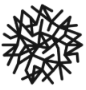
\includegraphics[width=0.23\textwidth]{imag/redes}
}
\clearpage
\bibliographystyle{ieeetran}
\bibliography{References}
\end{document}
